\documentclass[12pt,a4paper]{article}

\usepackage[margin=1in]{geometry}
\usepackage{microtype}
\usepackage{setspace}
\usepackage{enumitem}
\usepackage{booktabs}
\usepackage{array}
\usepackage{longtable}
\usepackage{graphicx}
\usepackage{xcolor}
\usepackage{titlesec}
\usepackage{fancyhdr}
\usepackage{tikz}
\usetikzlibrary{arrows.meta,positioning,shapes.geometric,fit}
\usepackage[colorlinks=true,linkcolor=black,urlcolor=blue!50!black]{hyperref}

\definecolor{accent}{HTML}{1F3A5F}
\definecolor{lightgrey}{HTML}{F2F4F7}

\setstretch{1.15}
\setlength{\parskip}{0.5em}
\setlength{\parindent}{0pt}

\titleformat{\section}{\Large\bfseries\color{accent}}{\thesection}{0.6em}{}
\titleformat{\subsection}{\large\bfseries\color{accent}}{\thesubsection}{0.6em}{}

\pagestyle{fancy}
\fancyhf{}
\fancyhead[L]{\small InfraDesk -- Project Synopsis}
\fancyhead[R]{\small Offline IT Support and Asset Management}
\fancyfoot[C]{\thepage}
\renewcommand{\headrulewidth}{0.4pt}

\newcommand{\fillin}[1]{\textbf{[#1]}}

\begin{document}

%-------------------------------------------------------------------
% TITLE PAGE
%-------------------------------------------------------------------
\begin{titlepage}
\centering
\vspace*{1.5cm}

{\Huge\bfseries\color{accent} INFRADESK\par}
\vspace{0.6cm}
{\Large\bfseries Offline IT Asset Management and\\ Problem Reporting System\\ with DevOps Automation\par}
\vspace{1.2cm}

{\large PROJECT SYNOPSIS\par}
\vspace{0.4cm}
{\normalsize Submitted in partial fulfilment of the requirements of the course\par}
{\normalsize \fillin{Course name and code}\par}

\vspace{2cm}

\begin{tabular}{>{\bfseries}l l}
Student Name        & \fillin{Your full name} \\[4pt]
Registration No.    & \fillin{Your registration / roll number} \\[4pt]
Programme / Branch  & \fillin{Programme, branch, semester} \\[4pt]
Institution         & \fillin{College / university name} \\[4pt]
Guide / Instructor  & \fillin{Instructor name} \\[4pt]
Date of Submission  & October 2026 \\
\end{tabular}

\vfill
{\small Items in square brackets must be completed by the student before submission.\par}
\end{titlepage}

%-------------------------------------------------------------------
\tableofcontents
\newpage

%-------------------------------------------------------------------
\section{Abstract}
Small laboratories, student project teams and local IT support groups often record technical problems on paper, in chat messages or in spreadsheets. Such records are easily lost, assignments are unclear and nobody can say who is working on which fault. At the same time, an application that is installed by hand on one computer is difficult to reproduce and may fail without anyone noticing.

\textbf{InfraDesk} is a locally hosted web application in which an administrator manages users, assets and tickets while workers report problems, receive assignments, add work notes and resolve tickets. All data is stored in a local SQLite database, and no paid or cloud service is needed at run time. The application is packaged in Docker containers and surrounded by a DevOps toolchain with clearly separated responsibilities: \textbf{Terraform} declares the local Docker infrastructure, \textbf{Puppet} enforces the configuration of an Ubuntu host, \textbf{Ansible} deploys and validates the application, and \textbf{Nagios Core} monitors its health endpoint and reports failures.

The project therefore combines a practical full-stack application with a reproducible deployment and monitoring workflow.

%-------------------------------------------------------------------
\section{Introduction and Background}
IT support is a routine need in computer laboratories, hostels, small offices and student teams. Commercial IT service management products exist, but they are costly, heavy to install and far larger than the needs of a small group. Free alternatives often require a database server, a mail server or a cloud account.

DevOps practice adds a second concern: how the application is installed, configured, updated and watched. Infrastructure as Code, configuration management, automated deployment and monitoring are normally taught separately. InfraDesk uses one small but real application as the subject of all four, so that each tool has a concrete and demonstrable purpose.

%-------------------------------------------------------------------
\section{Problem Statement}
\begin{enumerate}[leftmargin=*]
  \item Technical problems are reported informally, so there is no reliable history, ownership or status.
  \item There is no simple, free, offline tool for a small group to track tickets and local equipment.
  \item Manual installation is inconsistent from one machine to another and difficult to repeat.
  \item Host configuration can drift away from the intended state without being noticed.
  \item A stopped or unhealthy application is detected only when a user complains.
\end{enumerate}

%-------------------------------------------------------------------
\section{Objectives}
\begin{enumerate}[leftmargin=*]
  \item Build a role-based web application (Admin and Worker) for reporting, assigning, tracking and resolving IT support tickets.
  \item Maintain a simple, manually entered register of local assets and allow tickets to refer to them.
  \item Provide in-app notifications, ticket history, dashboards, reports and CSV export computed from real database records.
  \item Run entirely on one computer without internet access once dependencies have been downloaded.
  \item Package the system in Docker and provide a repeatable deployment.
  \item Use Terraform, Puppet, Ansible and Nagios Core for distinct, documented and demonstrable DevOps tasks.
  \item Verify the system with automated tests and report only results that were actually obtained.
\end{enumerate}

%-------------------------------------------------------------------
\section{Scope and Limitations}
\subsection{In scope}
Login and role-based authorization; ticket creation, assignment, status workflow, comments and history; in-app notifications; user and asset management; reports and CSV export; health and readiness endpoints; backup and restore of the database; Docker packaging; and the four DevOps components listed above.

\subsection{Out of scope}
InfraDesk is a student prototype and a local support tool. It is \emph{not} an emergency dispatch system, a production ITSM product or a remote monitoring agent. It does not discover devices automatically, does not send e-mail, SMS or push notifications, and does not claim that every failure is repaired automatically. Nagios detects and reports failures; recovery is performed by a documented, human-triggered Ansible procedure unless a tested event handler is explicitly added.

\subsection{Security notice}
The prototype is intended for a trusted local network. It must not be exposed directly to the public internet without a security review. SQLite is suitable for this single-computer prototype; a production deployment with many concurrent users would require a server database such as PostgreSQL.

%-------------------------------------------------------------------
\section{Proposed System}
\subsection{Users and Roles}
\begin{center}
\begin{tabular}{@{}p{2.2cm}p{12cm}@{}}
\toprule
\textbf{Role} & \textbf{Permissions}\\
\midrule
Admin  & Manage users, tickets, assignments, priorities and statuses; maintain the asset register; view reports, activity history and CSV export.\\
Worker & Report problems, see own and assigned tickets, add work notes, update permitted statuses, resolve tickets with a resolution note, read notifications.\\
\bottomrule
\end{tabular}
\end{center}
All permissions are enforced on the backend; the frontend only reflects them.

\subsection{Main Modules}
\begin{itemize}[leftmargin=*]
  \item \textbf{Authentication:} salted password hashing, short-lived signed tokens, inactive-account blocking.
  \item \textbf{Ticket workflow:} statuses OPEN, ASSIGNED, IN\_PROGRESS, WAITING, RESOLVED, CLOSED and CANCELLED with validated transitions; priorities LOW to URGENT; categories such as Hardware, Software, Network, Printer and Account Access.
  \item \textbf{Comments and history:} every comment, assignment and status change is stored as an event.
  \item \textbf{Notifications:} in-app, generated by real actions such as assignment, comment and status change.
  \item \textbf{Asset register:} asset tag, name, type, location, serial number, status and notes.
  \item \textbf{Dashboards and reports:} counts by status, priority, category and assignee computed from the database.
  \item \textbf{Operations:} \texttt{/health} and \texttt{/ready} endpoints, backup and restore scripts.
\end{itemize}

\subsection{Ticket Status Workflow}
\begin{center}
\begin{tabular}{@{}ll@{}}
\toprule
\textbf{From} & \textbf{Allowed next status}\\
\midrule
OPEN        & ASSIGNED, IN\_PROGRESS, CANCELLED\\
ASSIGNED    & IN\_PROGRESS, WAITING, CANCELLED\\
IN\_PROGRESS& WAITING, RESOLVED\\
WAITING     & IN\_PROGRESS, RESOLVED\\
RESOLVED    & CLOSED, IN\_PROGRESS (reopen)\\
CLOSED      & IN\_PROGRESS (reopen, admin only)\\
\bottomrule
\end{tabular}
\end{center}

%-------------------------------------------------------------------
\section{System Architecture}
\begin{center}
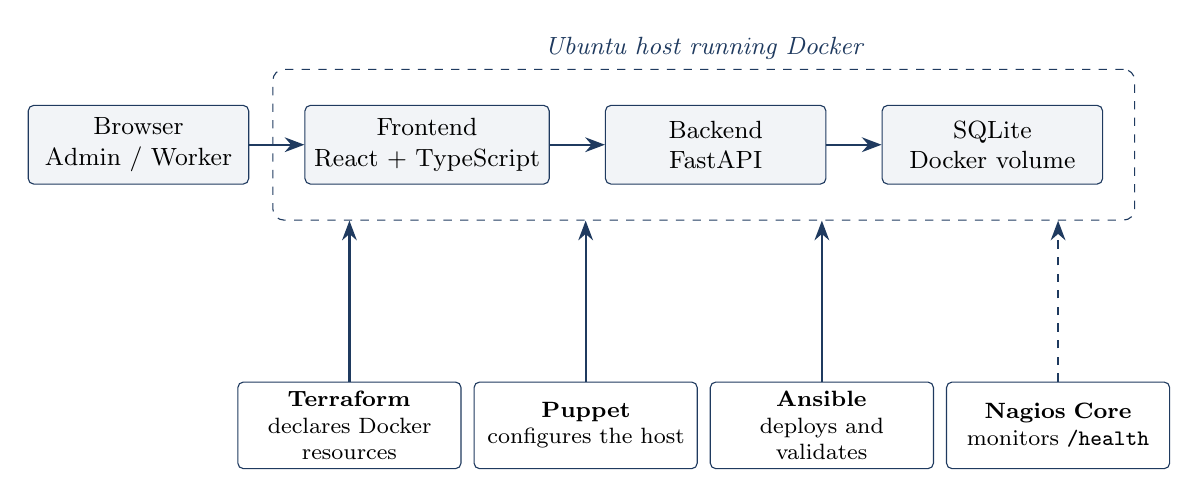
\begin{tikzpicture}[
  node distance=0.7cm,
  box/.style={rectangle,draw=accent,fill=lightgrey,rounded corners=2pt,minimum width=2.8cm,minimum height=1.0cm,align=center,font=\small},
  tool/.style={rectangle,draw=accent,fill=white,rounded corners=2pt,text width=2.6cm,minimum height=1.1cm,align=center,font=\footnotesize},
  host/.style={rectangle,draw=accent,dashed,rounded corners=4pt,inner xsep=0.4cm,inner ysep=0.45cm},
  arr/.style={-{Stealth[length=2.5mm]},thick,accent}
]
\node[box] (browser) {Browser\\Admin / Worker};
\node[box,right=of browser] (front) {Frontend\\React + TypeScript};
\node[box,right=of front] (api) {Backend\\FastAPI};
\node[box,right=of api] (db) {SQLite\\Docker volume};
\node[host,fit=(front)(api)(db),label={[font=\small\itshape,text=accent]above:Ubuntu host running Docker}] (hostbox) {};

\node[tool] (terraform) at ([xshift=-4.5cm,yshift=-2.6cm]hostbox.south) {\textbf{Terraform}\\declares Docker resources};
\node[tool] (puppet)    at ([xshift=-1.5cm,yshift=-2.6cm]hostbox.south) {\textbf{Puppet}\\configures the host};
\node[tool] (ansible)   at ([xshift=1.5cm,yshift=-2.6cm]hostbox.south)  {\textbf{Ansible}\\deploys and validates};
\node[tool] (nagios)    at ([xshift=4.5cm,yshift=-2.6cm]hostbox.south)  {\textbf{Nagios Core}\\monitors \texttt{/health}};

\draw[arr] (browser) -- (front);
\draw[arr] (front) -- (api);
\draw[arr] (api) -- (db);
\foreach \t in {terraform,puppet,ansible}
  \draw[arr] (\t.north) -- (\t.north |- hostbox.south);
\draw[arr,dashed] (nagios.north) -- (nagios.north |- hostbox.south);
\end{tikzpicture}
\end{center}

\noindent\textit{Figure 1.} The top row shows the request path of the application. Each tool in the bottom row acts on the Ubuntu and Docker environment that hosts it; the dashed arrow marks monitoring, which only observes and reports.

\subsection{Division of Responsibility}
\begin{center}
\begin{tabular}{@{}>{\bfseries}p{2.6cm}p{5.2cm}p{6.2cm}@{}}
\toprule
Tool & Responsibility & Demonstration\\
\midrule
Docker Compose & Simple development and demo run & Start application with a few commands; data survives restarts\\
Terraform & Declares the local Docker network, volume and containers in its own deployment mode & \texttt{init}, \texttt{validate}, \texttt{plan}, \texttt{apply}, \texttt{destroy}\\
Puppet & Baseline of the Ubuntu host: packages, directories, configuration files, service & Run twice for idempotence; change a managed file, re-run, show correction\\
Ansible & Preflight checks, deployment, validation, recovery & Playbook runs with handlers and a health check\\
Nagios Core & Monitors host and the \texttt{/health} endpoint & OK $\rightarrow$ CRITICAL when stopped $\rightarrow$ OK after recovery\\
\bottomrule
\end{tabular}
\end{center}
Terraform and Docker Compose are separate modes and never manage the same containers at the same time.

%-------------------------------------------------------------------
\section{Technology Stack}
\begin{center}
\begin{tabular}{@{}>{\bfseries}p{3.2cm}p{10.5cm}@{}}
\toprule
Layer & Technology\\
\midrule
Frontend & React, TypeScript, Vite, plain CSS (no external CDN, no icon library)\\
Backend & Python, FastAPI, Pydantic, SQLAlchemy, Alembic, Uvicorn\\
Database & SQLite on a persistent Docker volume\\
Security & Password hashing, signed tokens, backend role checks, narrow CORS\\
Packaging & Docker, Docker Compose\\
Infrastructure as Code & Terraform (Docker provider)\\
Configuration management & Puppet (\texttt{puppet apply} on an Ubuntu host or VM)\\
Deployment automation & Ansible\\
Monitoring & Nagios Core\\
Testing & pytest, Vitest and React Testing Library\\
Source control & Git and GitHub\\
\bottomrule
\end{tabular}
\end{center}
All tools are free and open source. No paid cloud service, paid API, map, SMS or e-mail service is required.

%-------------------------------------------------------------------
\section{Database Design}
The core tables are listed below.
\begin{center}
\begin{tabular}{@{}>{\ttfamily}p{3.4cm}p{10.3cm}@{}}
\toprule
\textrm{\textbf{Table}} & \textbf{Purpose}\\
\midrule
users             & Accounts, hashed passwords, role, active flag\\
tickets           & Support tickets with readable number (for example HD-000001), status, priority, category, reporter, assignee, optional asset\\
ticket\_comments  & Work notes and comments\\
ticket\_history   & Event log of assignments, status changes and comments\\
notifications     & In-app notifications with read state\\
assets            & Local equipment register\\
\bottomrule
\end{tabular}
\end{center}
Timestamps are stored in UTC. Foreign keys protect history; records referenced by history are archived or retired rather than deleted.

%-------------------------------------------------------------------
\section{Methodology}
Development follows twelve ordered phases. The application must work after every phase before the next one starts.
\begin{enumerate}[leftmargin=*]
  \item Foundation: repository, configuration, database, health endpoints.
  \item Authentication and role-based authorization, with tests.
  \item Ticket workflow, comments, history and notifications, with tests.
  \item User management, assets, reports and CSV export.
  \item Responsive frontend connected to the real API.
  \item Docker images and Compose with persistent storage.
  \item Terraform deployment mode.
  \item Puppet host configuration.
  \item Ansible preflight, deploy, validate and recovery.
  \item Nagios monitoring and failure demonstration.
  \item Offline operation, backup and restore verification.
  \item Documentation, report, demonstration script and viva preparation.
\end{enumerate}

%-------------------------------------------------------------------
\section{Testing and Evaluation Plan}
\begin{itemize}[leftmargin=*]
  \item \textbf{Backend tests:} login, inactive users, role boundaries, ticket persistence, transition rules, notifications, assets, reports, CSV escaping, input validation.
  \item \textbf{Frontend tests:} login validation, protected routes, role-aware navigation, form validation, loading, error and empty states.
  \item \textbf{DevOps checks:} Docker build, Compose validation, \texttt{terraform validate}, Puppet syntax check and repeat run, \texttt{ansible-playbook --syntax-check}, Nagios configuration test.
  \item \textbf{Failure demonstration:} stop the application and confirm that Nagios reports CRITICAL, then restore and confirm OK.
  \item \textbf{Operational checks:} backup and restore of a disposable database; operation with the internet disconnected after dependencies have been cached.
\end{itemize}
Results will be recorded exactly as obtained. A check that cannot be run in a given environment will be listed as \emph{not run} together with the reason.

%-------------------------------------------------------------------
\section{Hardware and Software Requirements}
\begin{center}
\begin{tabular}{@{}>{\bfseries}p{4cm}p{9.7cm}@{}}
\toprule
Item & Requirement\\
\midrule
Computer & Windows 11 laptop, 8~GB RAM, Ryzen 5 class CPU; no GPU needed\\
Operating systems & Windows 11 with Docker Desktop (WSL2), and Ubuntu 22.04/24.04 (VM or native) for the DevOps demonstration\\
Software & Docker, Git, Python 3.11+, Node.js 20+, Terraform, Puppet, Ansible, Nagios Core\\
Network & Internet only for first-time downloads; afterwards a local network is sufficient\\
\bottomrule
\end{tabular}
\end{center}

%-------------------------------------------------------------------
\section{Expected Outcomes}
\begin{itemize}[leftmargin=*]
  \item A working offline ticketing and asset register application with Admin and Worker portals.
  \item A repository that can be started with a small number of documented commands.
  \item Four demonstrable DevOps components with clear ownership boundaries.
  \item Automated test suites and honest, reproducible test records.
  \item Documentation: architecture, workflow, database design, API reference, security notes, installation guides, troubleshooting, demonstration script and viva preparation.
\end{itemize}

%-------------------------------------------------------------------
\section{Future Enhancements}
Optional e-mail notification through a local mail server, PostgreSQL for multi-user production use, file attachments with validation, rate limiting, and a tested Nagios event handler for narrowly scoped automatic recovery.

%-------------------------------------------------------------------
\section{Project Plan (Estimate)}
\begin{center}
\begin{tabular}{@{}>{\bfseries}p{1.3cm}p{9.5cm}p{3cm}@{}}
\toprule
Phase & Activity & Estimated effort\\
\midrule
1--2  & Foundation, authentication, roles & \fillin{days}\\
3--4  & Tickets, users, assets, reports & \fillin{days}\\
5     & Frontend & \fillin{days}\\
6--7  & Docker and Terraform & \fillin{days}\\
8--10 & Puppet, Ansible, Nagios & \fillin{days}\\
11--12& Offline checks, documentation, report & \fillin{days}\\
\bottomrule
\end{tabular}
\end{center}
Durations are to be estimated by the student according to the available schedule.

%-------------------------------------------------------------------
\section{References}
\begin{enumerate}[label={[\arabic*]},leftmargin=*]
  \item FastAPI documentation. \url{https://fastapi.tiangolo.com}
  \item SQLAlchemy documentation. \url{https://docs.sqlalchemy.org}
  \item React documentation. \url{https://react.dev}
  \item Docker documentation. \url{https://docs.docker.com}
  \item Terraform documentation, Docker provider. \url{https://developer.hashicorp.com/terraform/docs}
  \item Puppet documentation. \url{https://www.puppet.com/docs/puppet}
  \item Ansible documentation. \url{https://docs.ansible.com}
  \item Nagios Core documentation. \url{https://www.nagios.org/documentation}
\end{enumerate}

\vspace{1.2cm}
\begin{tabular}{@{}p{7cm}p{7cm}@{}}
Signature of Student: \rule{4cm}{0.4pt} & Signature of Guide: \rule{4cm}{0.4pt}\\[10pt]
Date: \rule{4cm}{0.4pt} & Date: \rule{4cm}{0.4pt}\\
\end{tabular}

\end{document}
